\section*{Appendix A: Sample Calcs}

\begin{enumerate}[wide,label=\textbf{\arabic*}., labelindent=0pt]

    \item \textbf{Wing Loading}
        \[WS = \frac{W}{S_ref}\]
        $ W =$ weight [oz]\\
        $S_ref =$ strain in the $x$ direction after the transformation\\
        $\epsilon_y' =$ strain in the $x$ direction after the transformation\\
        
        \underline{For an aluminum beam in bending with a force of 8.90 N at Rosette 1:} \\
        \begin{align*}
            \gamma_{xy} &= (4.0 \times 10^{-6}) - (4.0 \times 10^{-6})\\
            &= 0.0 \times 10^{-6}\\
        \end{align*}
 
\section*{Appendix B: Engineering Drawings}\label{ApxB}   
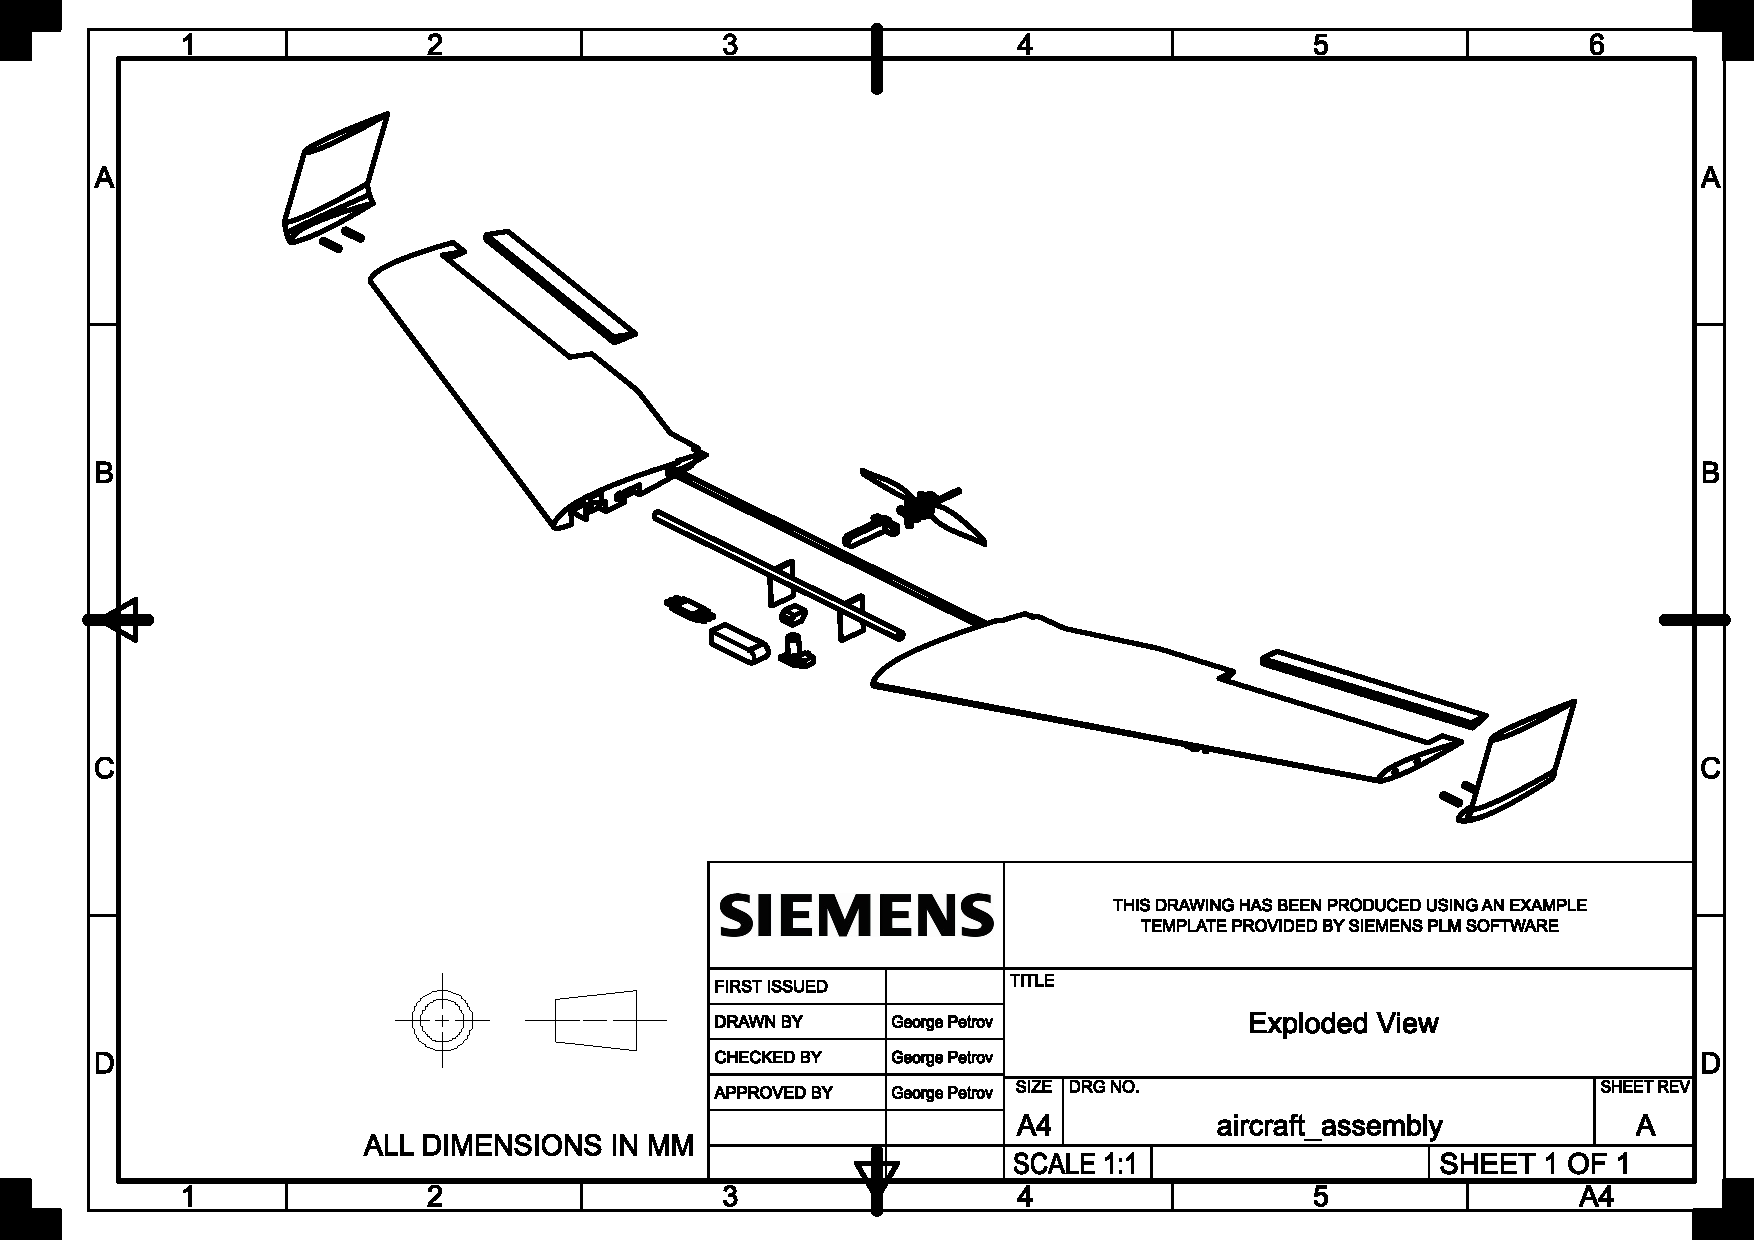
\includepdf[pages=-,angle=90]{homeworks/homework4/report/Figure/gpetrov2_aircraft_assembly_exploded_drawing.pdf}
\end{enumerate}